
\section[Miscellaneous]{Miscellaneous}
\label{sec:misc}
\addcontentsline{toc}{section}{\thesection. Miscellaneous}

\code{fitMultinom()} is an utility function which can fit a ROC model with
$\phi$ values assuming no measurement errors as in~\cite{Shah2011}.
A typical usage is as the following
\begin{Code}
> demo(fitMultinom, 'cubfit')
\end{Code}
or
\begin{Code}
> rm(list = ls())
>
> suppressMessages(library(cubfits, quietly = TRUE))
>
> # fit Shah & Gilchrist (2011)
> init.function(model = "roc")
> fitlist <- fitMultinom(ex.train$reu13.df, ex.train$phi.Obs,
+                        ex.train$y, ex.train$n)
> ret.fit <- prop.model.roc(fitlist, phi.Obs.lim = range(phi.Obs))
>
> # plot.
> par(mfrow = c(1, 3))
> for(i.aa in 1:length(aa.list)){
>   plotmodel(ret.model = ret.fit[[i.aa]], main = aa.list[i.aa])
> }
\end{Code}
where \code{fitlist} is an object of \code{b} data structure containing
all estimations of $(log(\mu), \Delta t)$ for each synonymous codon and
amino acid.
This is a quick fit assuming no measurement error on expression levels.
This demo returns plots in Figure~\ref{fig:fitMultinom}
\begin{figure}[ht]
\centering
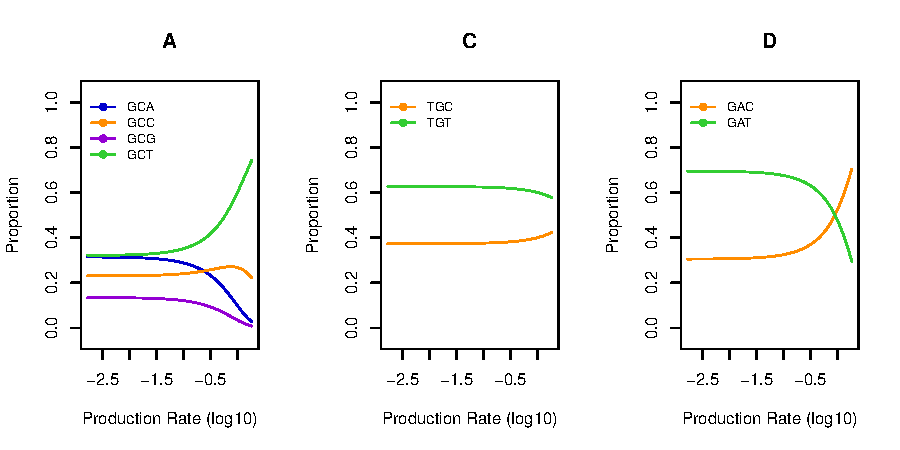
\includegraphics[width=6in]{cubfits-include/figure/fitMultinom}
\caption{A simple prediction plot, similar to Figure~\ref{fig:plotbin}
except empirical binning.
}
\label{fig:fitMultinom}
\end{figure}

{\color{red} \bf Important:}
Note that \code{init.function(model = "roc")} is to initial generic functions
for the ROC model and \code{fitMultinom()} can access corresponding generic
functions from environment \code{.cubfitsEnv}. The generic function then
perform multinomial logistic regression on the input summarized statistics,
and \code{VGAM::vglm()} can fit and return parameter estimations.
Therefore, there is only need to initial once before MCMC iterations, such as
the three main function in Section~\ref{sec:main_functions}. For performance
issue, all calls within MCMC iterations should access generic functions, such
as via \code{.cubfitEnv$fitMultinom()} regardless models. Do *NOT*
access this function, \code{fitMultinom()}, within any MCMC iteration.

